\documentclass[12pt, a4paper]{exam}
\usepackage{graphicx}
\usepackage[left=0.8in, top=0.7in, total={6.2in,10in}]{geometry}
\usepackage[normalem]{ulem}
\usepackage{comment}
\usepackage{amsmath}
\usepackage{float}

\renewcommand\ULthickness{1.0pt}   %%---> For changing thickness of underline
\setlength\ULdepth{1.3ex}%\maxdimen ---> For changing depth of underline

%% HEADER
\begin{document}
	\noindent
	\begin{minipage}[l]{0.1\textwidth}
		\noindent
		
\includegraphics[width=1.8\textwidth]{res/iiserb_logo.png}
	\end{minipage}
\hfill
\begin{minipage}[c]{0.8\textwidth}
	\begin{center}
		{\large	Indian Institute of Science Education and Research Bhopal \par
		\large	\par
	\large \textbf{	Computer Vision( DSE/EECS-312)}	\par
\small	Assignment-1: Answer Sheet}
	\end{center}
\end{minipage}

%% FIELDS AND INSTRUCTIONS
\par
\vspace{0.2in}
\noindent
\textbf{Name: }Adheesh Trivedi\\
\noindent
\textbf{Roll No.:  }22016\\
\noindent
\uline{\textbf{Time of submission: } \hfill 		\hfill Marks Obtained: } \\
\uline{Please follow the instructions given in the assignment carefully. \hfill}
\par 
\vspace{0.15in}
\noindent
\centering
{\small \bfseries  Please provide your detailed answers and any explanations or diagrams directly below each question in the 'Answers' section. }

%% QUESTIONS
\vspace{0.2in}
\begin{questions}
	\pointsdroppedatright

%% QUESTION 1
	\question
Apply the filters mentioned below on the image attached and analyze their impact.
Describe what you found after applying each filter
and why certain phenomena are happening. \textbf{\textit{(Marks: )}}\\

\begin{enumerate}

\item \begin{center}
\begin{tabular}{|c|c|c|}
\hline
-1 & 0 & 1 \\ \hline
-1 & 0 & 1 \\ \hline
-1 & 0 & 1 \\ \hline
\end{tabular}
\end{center}

\item \begin{center}
\begin{tabular}{|c|c|c|}
\hline
1 & 1 & 1 \\ \hline
0 & 0 & 0 \\ \hline
-1 & -1 & -1 \\ \hline
\end{tabular}
\end{center}

\end{enumerate}

Since the above filters are of dimension $3 \times 3$. Construct the same filters of dimension $5 \times 5$ and do the above experiments.
\vspace{0.2in}
    \pointsdroppedatright\\

%% ANSWER 1
\textbf{Answer:}

\textbf{Prewitt filter (3 by 3)}

I used the $3\times3$ Prewitt filter to produce image dipicting the edges in the original image:

$$\delta_x = \frac{1}{3}
\begin{bmatrix}
    -1 & 0 & 1 \\
    -1 & 0 & 1 \\
    -1 & 0 & 1
\end{bmatrix}$$

and,

$$\delta_y = \frac{1}{3}
\begin{bmatrix}
-1 & -1 & -1 \\
0 & 0 & 0 \\
1 & 1 & 1
\end{bmatrix}$$

These filters when convolved with the original image gives the following images:

\begin{figure}[H]
    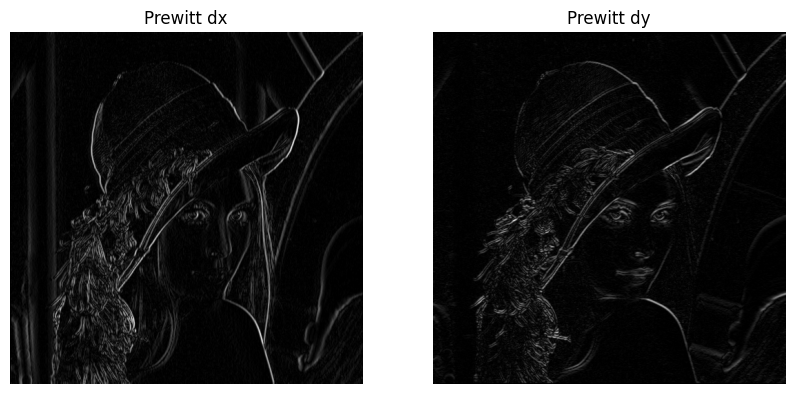
\includegraphics[width=1.06\textwidth]{res/1_prewitt.png}
    \caption{Prewitt filter applied to the original image}\label{fig:1_prewitt}
\end{figure}

Here we notice that the images is highlighting the edges that were in the orignial image.

\textbf{Comparision with larger filter (5 by 5)}

I used the following $5\times5$ filter to produce image dipicting the edges in the original image:

$$\delta_x = \frac{1}{15}
\begin{bmatrix}
-1 & -2 & 0 & 2 & 1 \\
-1 & -2 & 0 & 2 & 1 \\
-1 & -2 & 0 & 2 & 1 \\
-1 & -2 & 0 & 2 & 1 \\
-1 & -2 & 0 & 2 & 1
\end{bmatrix}$$

and,

$$\delta_y = \frac{1}{15}
\begin{bmatrix}
-1 & -1 & -1 & -1 & -1 \\
-2 & -2 & -2 & -2 & -2 \\
0 & 0 & 0 & 0 & 0 \\
2 & 2 & 2 & 2 & 2 \\
1 & 1 & 1 & 1 & 1
\end{bmatrix}$$

Here the 2nd and 2nd last enteries have greater value than the first and the last enteries. This is because the center pixel has more weightage than the pixels at the corners. This is done to increase localization in the gradient.

\begin{figure}[H]
    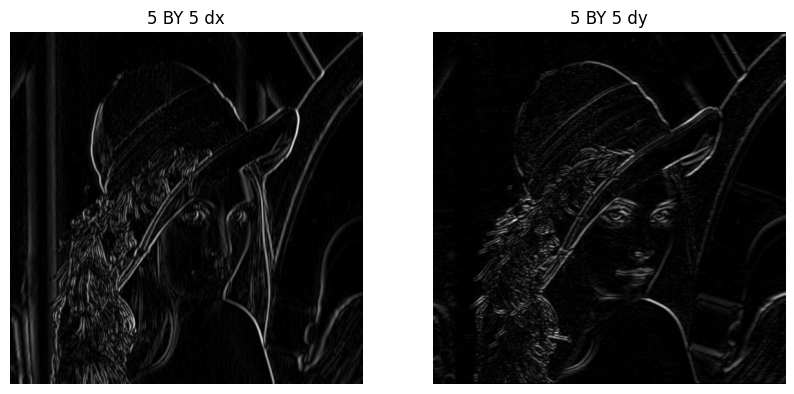
\includegraphics[width=1.06\textwidth]{res/1_5_by_5.png}
    \caption{5 by 5 filter applied to the original image}\label{fig:1_5by5}
\end{figure}

\textbf{Results}

The $\delta_x$ filter detects vertical edges and the $\delta_y$ filter detects horizontal edges. This is happening because the filter computes gradient about the direction mentioned in its subscript. So when there is sudden change in the pixel values in the direction of the filter, the filter gives a high value. Since edges are nothing but sudden changes in a function. This is why the edges are highlighted in the images.

Few differences observed between different size of filters:

\begin{itemize}
    \item The edges are thicker in $5\times5$ than in $3\times3$.
    \item $3\times3$ does a lot better in preserving the hair details.
\end{itemize}

\vspace{0.2in}

\newpage
%% QUESTION 2
	\question
 Sobel Edge Detection Implementation. \textbf{\textit{(Marks: )}}
\begin{parts}
    \part[9] Write a Python function to apply the Sobel filter given below to detect edges along the x-direction and y-direction. Combine these to compute the gradient magnitude image.
    \begin{enumerate}

        \item \begin{tabular}{|c|c|c|}
\hline
-1 & 0 & 1 \\ \hline
-2 & 0 & 2 \\ \hline
-1 & 0 & 1 \\ \hline
\end{tabular} 
\item \begin{tabular}{|c|c|c|}
\hline
1 & 2 & 1 \\ \hline
0 & 0 & 0 \\ \hline
-1 & -2 & -1 \\ \hline
\end{tabular} 
\item \begin{tabular}{|c|c|c|c|c|}
\hline
1 & 2 & 3 & 2 & 1 \\ \hline
2 & 3 & 5  & 3 & 2 \\ \hline
0 & 0 & 0 & 0 & 0 \\ \hline
-2 & -3 & -5  & -3 & -2 \\ \hline
-1 & -2 & -3 & -2 & -1 \\ \hline
\end{tabular}
\item \begin{tabular}{|c|c|c|c|c|}
\hline
-1 & -2 & 0 & 2 & 1 \\ \hline
-2 & -3 & 0 &   3 & 2 \\ \hline
-3 & -5 & 0 & 5 & 3 \\ \hline
-2 & -3 & 0 & 3 & 2  \\ \hline
-1 & -2 & 0 & 2 & 1 \\ \hline
\end{tabular}

    \end{enumerate}
    \vspace{0.05in}
    \part[9] Apply your function to an image and display the gradient magnitude image alongside the original. Vary the size of the kernel and document the effects.
    \vspace{0.05in}
    \part[9] Manually implement thresholding on the gradient magnitude to create a binary edge image. Experiment with different thresholds and show the results.
    \vspace{0.05in} 
    \part[9] Apply the Sobel edge detector on a noisy image (you may add synthetic noise to an attached clean image). Discuss how noise affects edge detection and the visual quality of the output images.
\end{parts}

\vspace{0.2in}
\pointsdroppedatright

%% ANSWER 2
\textbf{Answer:}

\textbf{Loading dataset}

I loaded 500 images of real faces and 500 images of spoof faces from the dataset.

\textbf{Raw pixel values}

The raw pixel values of the face images are used as features. I trained a Support Vector Machine (SVM) classifier on these raw pixel features to classify fake and real faces. The performance of the model on the dataset is portrayed in the code.

\textbf{Local Binary Patterns (LBP) features}

Local Binary Patterns (LBP) features are extracted from the face images for feature extraction. I trained an SVM classifier using the LBP features to classify fake and real faces. The performance of the model on the dataset is portrayed in the code.

\begin{figure}[H]
    \centering
    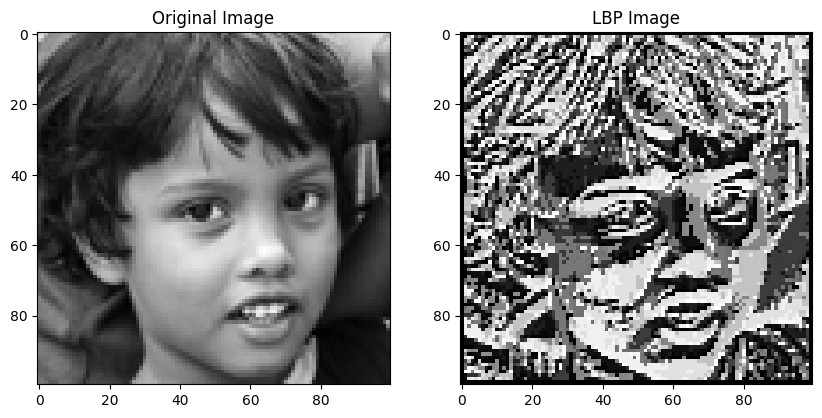
\includegraphics[width=.9\textwidth]{imgs/lbp.png}
    \caption{Local binary pattern}
    \label{fig:2_mediapipe}
\end{figure}

\newpage

\textbf{Edge methods}

Edge images are computed using the Prewitt and Sobel edge detectors. These edge images are used as input features independently to train an SVM classifier and classify fake and real faces. The performance of the model on the dataset is portrayed in the code.

\begin{figure}[H]
    \centering
    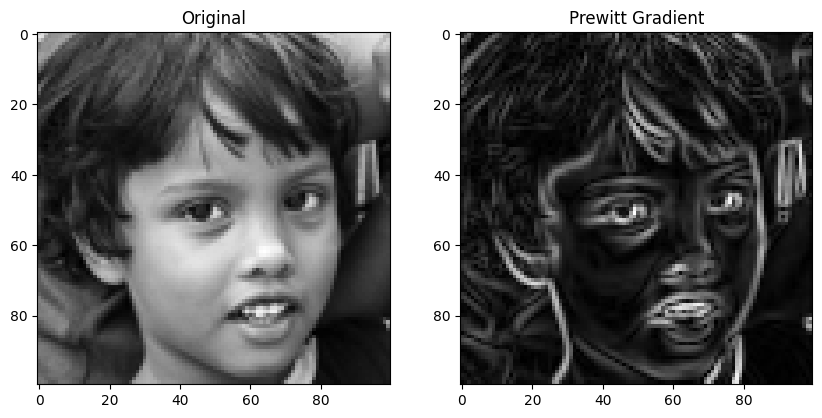
\includegraphics[width=.9\textwidth]{imgs/prewitt.png}
    \caption{Prewitt filtered image}
    \label{fig:2_mediapipe}
\end{figure}


\begin{figure}[H]
    \centering
    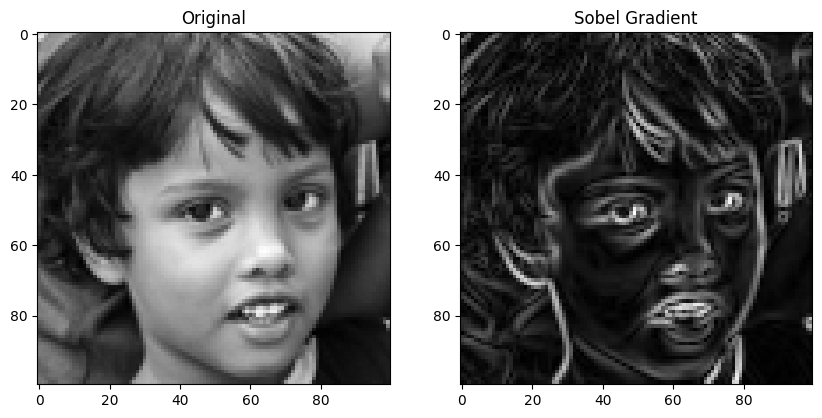
\includegraphics[width=.9\textwidth]{imgs/sobel.png}
    \caption{Sobel filtered image}
    \label{fig:2_mediapipe}
\end{figure}

\vspace{0.2in}
\newpage
%% QUESTION 3
	\question
Laplacian of Gaussian Edge Detection (follow the class notes).  \textbf{\textit{(Marks: )}}
\begin{parts}
    \part[9] Implement Gaussian smoothing from scratch. Apply your Gaussian filter given below to smooth an image before edge detection.

    \vspace{0.05in}
    \part[9] Develop the Laplacian filter and apply it to the smoothed image from 3 (a) to detect edges via zero-crossings. Describe how you detect zero-crossings in your implementation.
    \vspace{0.05in}
    \part[9] Display the edges detected from the smoothed image alongside the edges detected from the non-smoothed image. Discuss the differences and the impact of noise.
\end{parts}
\vspace{0.2in}

%% ANSWER 3
\textbf{Answer:}

{\large(a)}

\textbf{Gaussian filter and Gaussian blur}

I used the Gaussian filter to smoothen the image to reduce impact of noise in edge detection algorithms being used here. The Gaussian filter is used to blur the image. The filter is given by:

$$n_\sigma = \frac{1}{16} \times
\begin{bmatrix}
    1 & 2 & 1 \\
    2 & 4 & 2 \\
    1 & 2 & 1
\end{bmatrix}$$

This is reffered as Gaussian blur and is very often used in image processing.

\begin{figure}[H]
    \centering
    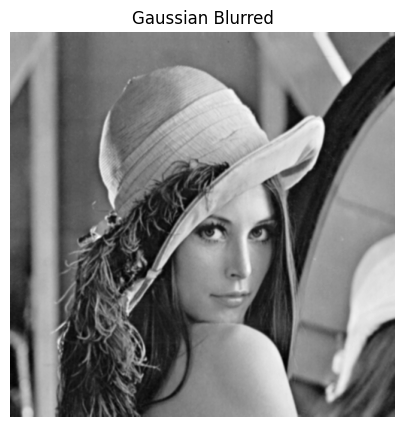
\includegraphics[width=.5\textwidth]{res/3a_gaussian.png}
    \caption{Gaussian filter applied to the original image}\label{fig:3a_gaussian}
    \label{fig:3d_gaussian}
\end{figure}

The result is slightly blurred as the kernel size is very small ($3\times3$). Image will get more blurry when we increase the kernel size, as the kernel would have more pixels to interact with.

{\large(b)}

\textbf{Laplacian filter}

The Laplacian filter is a second-order derivative filter used in image processing for edge detection and enhancement. It highlights regions of rapid intensity change, which correspond to edges in an image. I used the following laplacian filter that was taught in class:

$$\Delta^2 =
\begin{bmatrix}
    0 & 1 & 0 \\
    1 & -4 & 1 \\
    0 & 1 & 0
\end{bmatrix}$$

This filter is convolved with the image to produce the following image:

\begin{figure}[H]
    \centering
    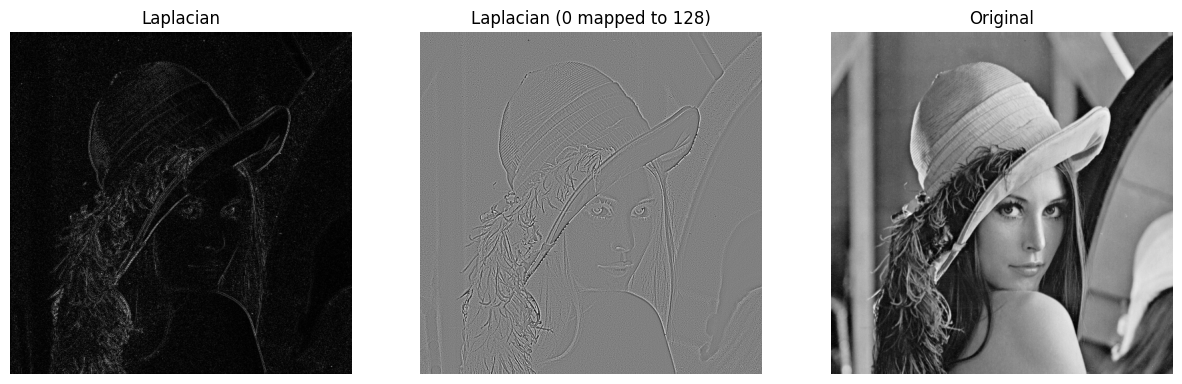
\includegraphics[width=1.06\textwidth]{res/3b_laplacian.png}
    \caption{Laplacian filter applied to the original image}
    \label{fig:3b_laplacian}
\end{figure}

\textbf{Zero crossing}

The way I implemented zero crossing here is for each pixel value $P_{i,j}$ I am checking if the sign is changed from previous pixels, that is $P_{i-1,j}$ and $P_{i,j-1}$. If the sign is changed then I am marking that pixel as edge pixel if the change between the pixels is greater than a certain threshold given to the function of zero crossing I have implemented.

As observed here, no matter how much I increase the zero crossing, the results are consistently noisy. This is because the image is noisy and the zero crossing is not able to detect the edges properly due to it's small size of kernel. Also, we would want to keep the threshold as low as possible, as more the threshold, more the edges will be lost.

\begin{figure}[H]
    \centering
    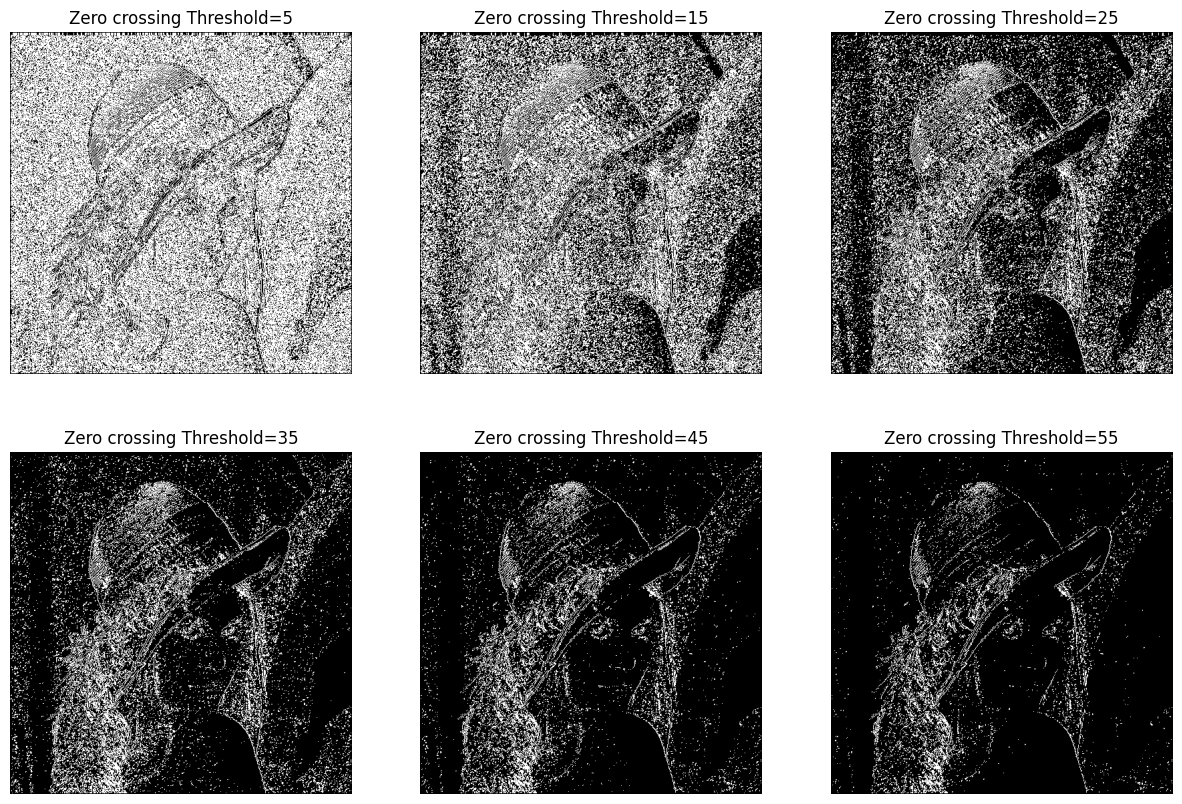
\includegraphics[width=1.06\textwidth]{res/3b_zero_crossing.png}
    \caption{Zero crossing applied to the laplacian image with different threshold}
    \label{fig:3b_zero_crossing}
\end{figure}

\textbf{Laplacian of Gaussian (LoG)}

To over come the issue of noise in the laplacian filtered image, we would want our main image to be our of noise, i.e., we want the original image to be smooth. This can be done using gaussian filter. The LoG is the convolution of the laplacian filter and the gaussian filter. The LoG is given by:

$$LoG*I = \Delta^2 * n_\sigma * I$$

\begin{figure}[H]
    \centering
    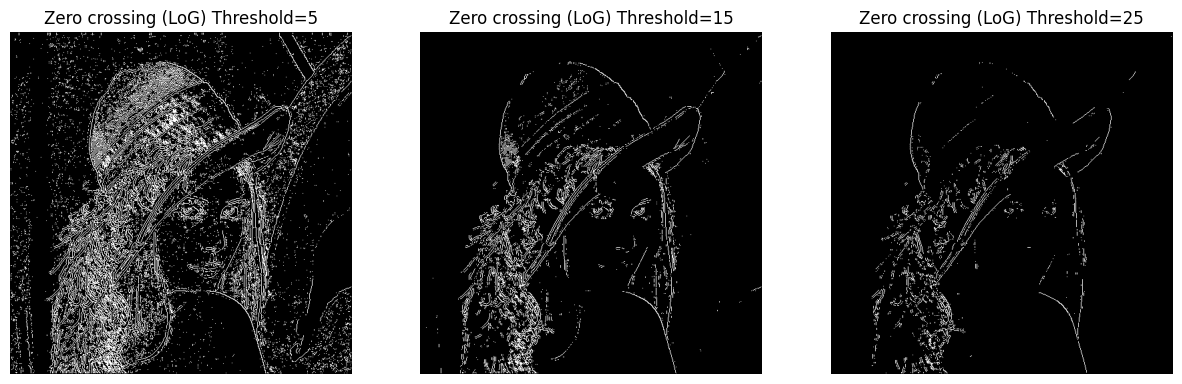
\includegraphics[width=1.06\textwidth]{res/3b_zero_crossing_log.png}
    \caption{LoG applied to the original image}
    \label{fig:3c_log}
\end{figure}

{\large(c)}

As you can see that we get very good results at $threshold=15$ only, compared to that of useless results with only laplacian filter. Here below is a side my side comparision of The original image, laplacian filter and LoG filter.

\begin{figure}
    \centering
    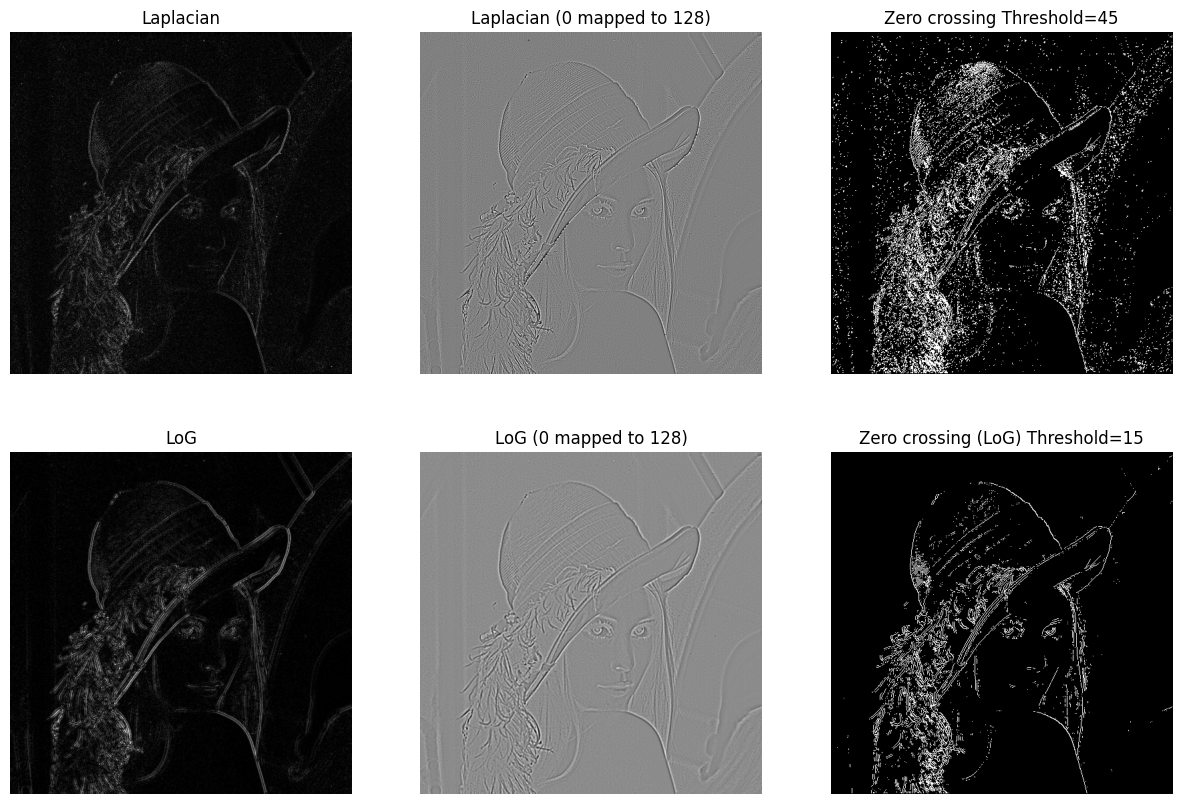
\includegraphics[width=1.06\textwidth]{res/3c_log_vs_lap.png}
    \caption{LoG vs Laplacian filter}
    \label{fig:3c_log_vs_lap}
\end{figure}

\vspace{0.2in}

\end{questions}

\end{document}